\documentclass[10pt,twocolumn,letterpaper]{article}

\usepackage{dependable_dnn}
\usepackage{times}
\usepackage{epsfig}
\usepackage{graphicx}
\usepackage{amsmath}
\usepackage{amssymb}
\usepackage{subfigure}
\usepackage[table, dvipsnames]{xcolor}

% Include other packages here, before hyperref.

% If you comment hyperref and then uncomment it, you should delete
% egpaper.aux before re-running latex.  (Or just hit 'q' on the first latex
% run, let it finish, and you should be clear).
\usepackage[pagebackref=true,breaklinks=true,letterpaper=true,colorlinks,bookmarks=false]{hyperref}

\iccvfinalcopy % *** Uncomment this line for the final submission

\def\iccvPaperID{} % *** Enter the Paper ID here
\def\httilde{\mbox{\tt\raisebox{-.5ex}{\symbol{126}}}}

% Pages are numbered in submission mode, and unnumbered in camera-ready
\ificcvfinal\pagestyle{empty}\fi
\newcommand{\N}{{\mathbf{N}}}  
\newcommand{\R}{{\mathbf{R}}}  
\newcommand{\A}{{\mathbf{W}}}   
\newcommand{\n}{{\mathbf{n}}}   
\newcommand{\argmax}{\mathop{\arg\max}}  % notation of argmax.

\begin{document}

%%%%%%%%% TITLE - PLEASE UPDATE
\title{Closed-Form Factorization of Latent Semantics in GANs\\ {\rm {\normalsize Seungmin Lee (profile2697@gmail.com; 2020-20866), \\Dept. of Electrical and Computer Engineering, Seoul National University}}}   % **** Enter the paper title and student information here

\maketitle
\thispagestyle{empty}

\section{Introduction}
The latent space of Generative Adversarial Network (GAN) has a rich set of interpretable directions that we can use to edit synthesized images. However, previous methods to find the interpretable directions require human annotations on a collection of synthesized images. In this paper, the authors propose a closed-form algorithm that identifies the semantic directions without using human annotations. More specifically, the proposed method discovers semantics by only using the weights of a pre-trained generator.

\section{Preliminaries: Manipulating Generator in GAN Latent Space}
A generator $G(\cdot)$ takes a $d$-dimensional latent vector $\mathbf{z}$ from the latent space $\mathcal{Z} \in \mathbf{R}^d$ and produces an image $\mathbf{I} = G(\mathbf{z})$. The authors focus on the first layer of the generator ($G_1\colon \mathbf{R}^d \to \mathbf{R}^m$) since it directly acts on the latent space. Like most many GANs have done, the authors assume $G_1$ is an affine transformation:
\begin{align*}
    \mathbf{y} := G_1(\mathbf{z}) = \mathbf{W}\mathbf{z} + \mathbf{b},
\end{align*}
where $\mathbf{W} \in \mathbf{R}^{m \times d}$ and $\mathbf{b} \in \mathbf{R}^m$ denote the weights and bias, respectively.

We can manipulate the image generation by adding a particular direction $\mathbf{n} \in \mathbf{R}^d$ that represents a semantic concept to a given input vector: 
\begin{align*}
    \text{edit}(G(\mathbf{z})) = G(\mathbf{z} + \alpha\mathbf{n})
\end{align*}
where $\alpha$ controls the manipulation intensity.

\section{Method}
At the first layer, we can simplify the manipulation as follows:
\begin{align}
    \mathbf{y}' &= G_1(\mathbf{z} + \alpha\mathbf{n}) = \mathbf{W}(\mathbf{z} + \alpha\mathbf{n}) + \mathbf{b}\nonumber\\
    &= (\mathbf{W}\mathbf{z} + \mathbf{b}) + \alpha\mathbf{W}\mathbf{n}\nonumber\\
    &= \mathbf{y} + \alpha\mathbf{W}\mathbf{n}.\label{eq}
\end{align}

By observing Eq.~(\ref{eq}), the authors claim that $\mathbf{W}$ already contains essential information about the image edition, and thus, we can discover useful latent directions by decomposing $\mathbf{W}$.

Assume that we want to find $k$ most significant directions $\N^{*} \in \mathbf{R}^{d \times k}$. Then, $\N^{*}$ should satisfy the following equation:
\begin{align}
    \N^* = \argmax_{\{\N\in\R^{d\times k}:\ \n_i^T\n_i = 1\ \forall i=1,\cdots,k\}} \sum_{i=1}^k ||\A\n_i||_2^2,  \label{eq:optimization}
\end{align}
where $\n_i \in \mathbf{R}^d$ denotes the $i$-th column of $\N$, and $||\cdot||_2$ corresponds to $l_2$ norm.

The authors use the Lagrange multipliers $\{\lambda_i\}_{i=1}^k$ to solve Eq.~(\ref{eq:optimization}). With the multipliers, Eq.~(\ref{eq:optimization}) can be written as:
\begin{align}
    \N^* &= \argmax_{\N\in\R^{d\times k}} \sum_{i=1}^k ||\A\n_i||_2^2 - \sum_{i=1}^k\lambda_i(\n_i^T\n_i - 1) \nonumber \\
    &= \argmax_{\N\in\R^{d\times k}} \sum_{i=1}^k (\n_i^T\A^T\A\n_i - \lambda_i\n_i^T\n_i + \lambda_i). \label{eq:lagrange}
\end{align}

By taking partial derivative of Eq.~(\ref{eq:lagrange}), we get $\n_i$:
\begin{align}
    2\A^T\A\n_i - 2\lambda_i\n_i = 0. \label{eq:solution}
\end{align} 

\section{Results}
The authors conduct experiments using various GANs. The proposed method consistently finds useful directions, as we can observe from Fig.~(\ref{fig:imgs}). 

\begin{figure}[h]
	\centering
	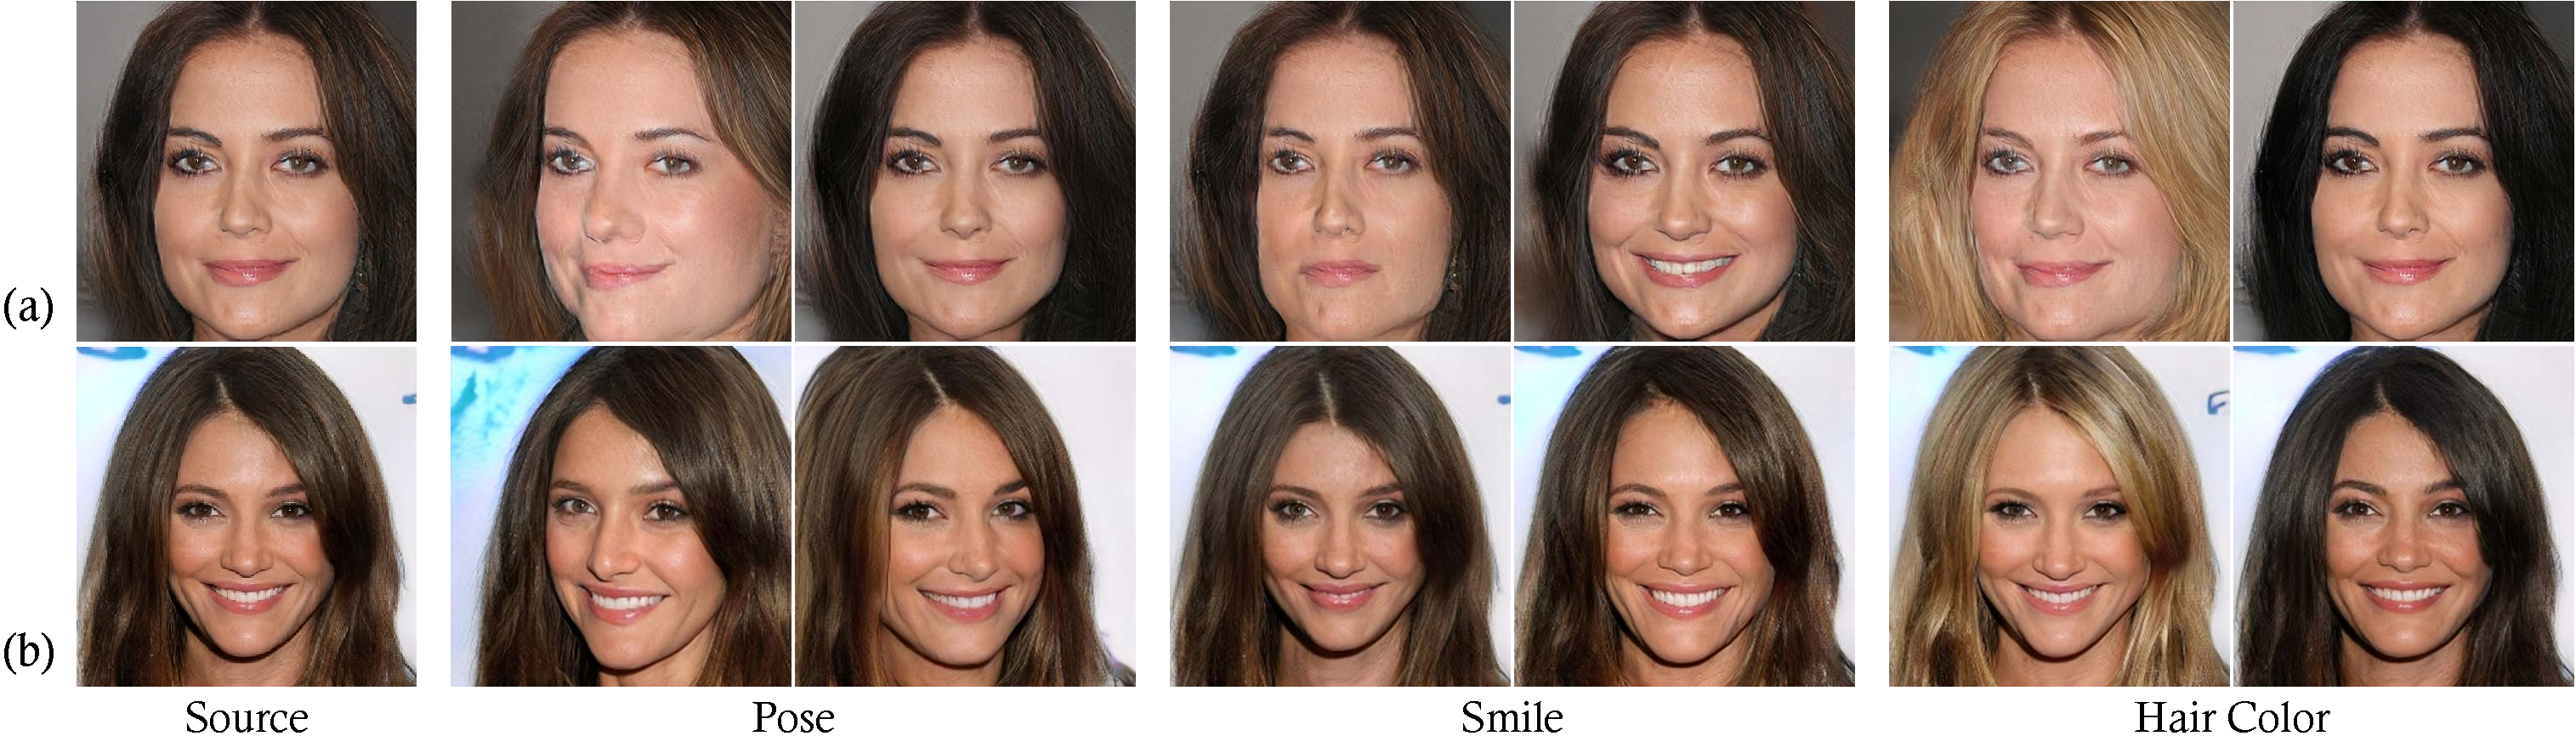
\includegraphics[width=8cm]{assets/comparison_infogan.pdf}
	\caption{Some qualitative results.}
	\label{fig:imgs}
\end{figure}

\section{Personal Note}
The authors' claims are intuitive and useful. Moreover, the proposed method seems practical since it does not require any data samples and human annotations. 

\end{document}
